\section{Results}
\label{sec:results}

\subsection{Baselines replicate; the hybrids do not}

Table~\ref{tab:r1} lists, for every dataset, the protocol-B (honest)
accuracy of the C4.5 and NB baselines and of Algorithms 1 and 2, next to
Farid et al.'s reported numbers. The C4.5 baseline is within 1.4 points of
the paper on 7 of the 9 non-NSL-KDD datasets (largest gap $-2.89$ on iris,
smallest 0.00 on diabetes), and the NB baseline is within 2.0 points on 7
of 10 datasets. NSL-KDD is the exception for C4.5: this replication scores
99.47\% against a reported 71.11\%, a 28.36-point gap far outside the
spread on any other dataset; we did not find a configuration change that
closes it and report it as unresolved rather than adjust the protocol
until it matches. The hybrids do not replicate on average: Algorithm~1
reaches a mean of 81.02\% against a reported 88.43\%, worst on glass
($-27.14$), and Algorithm~2 reaches 77.16\% against 83.42\%, worst on
NSL-KDD ($-19.66$). Table~\ref{tab:tests} shows neither honest hybrid
beats its baseline once Holm correction is applied: Algorithm~1 vs.\ C4.5
has a median difference of $-3.71$ points ($p=0.055$, Holm $p=0.328$), and
Algorithm~2 vs.\ NB has a median difference of $+0.65$ points ($p=0.164$,
Holm $p=0.656$). Neither result supports the paper's claim of a
consistent hybrid advantage under an evaluation protocol that never lets a
stage see a test instance's label.

% R1: Weka J48 (pruned) / FaithfulNB replication, protocol B honest, 10-fold CV x 3 seeds.
\begin{table*}[t]
\caption{R1 replication (protocol B, refit-per-fold): C4.5 and NB baselines and the two hybrids, against Farid et al.\ (2014).}
\label{tab:r1}
\centering\small
\begin{tabular}{lrrrrrrrr}
\toprule
& \multicolumn{2}{c}{C4.5} & \multicolumn{2}{c}{NB} & \multicolumn{2}{c}{Alg.\ 1} & \multicolumn{2}{c}{Alg.\ 2} \\
Dataset & ours & paper & ours & paper & ours & paper & ours & paper \\
\midrule
breast-cancer & 75.31 & 75.52 & 72.39 & 71.67 & 71.61 & 81.46 & 72.63 & 75.87 \\
contact-lenses & 85.00 & 83.33 & 73.33 & 70.83 & 85.00 & 91.66 & 79.44 & 87.50 \\
diabetes & 73.82 & 73.82 & 75.52 & 76.30 & 75.52 & 79.03 & 77.12 & 85.41 \\
glass & 66.88 & 66.82 & 46.60 & 48.59 & 49.13 & 76.27 & 47.41 & 52.33 \\
image-segmentation & 96.75 & 95.73 & 79.67 & 81.06 & 89.11 & 96.53 & 81.75 & 85.19 \\
iris & 93.11 & 96.00 & 95.56 & 96.00 & 94.67 & 98.66 & 95.56 & 98.00 \\
nsl-kdd & 99.47 & 71.11 & 67.44 & 76.27 & 86.57 & 81.92 & 62.73 & 82.39 \\
soybean & 92.54 & 91.50 & 89.94 & 92.83 & 88.82 & 92.97 & 89.40 & 94.15 \\
tic-tac-toe & 85.08 & 85.07 & 69.87 & 69.62 & 74.50 & 88.10 & 70.36 & 78.91 \\
vote & 94.93 & 96.32 & 90.18 & 90.11 & 95.25 & 97.70 & 95.24 & 94.48 \\
\bottomrule
\end{tabular}
\end{table*}


\subsection{Fitting the filter before cross-validation inflates Algorithm 1}

Table~\ref{tab:tests} reports the protocol-A-vs-B comparison directly.
Under R1's Weka/J48 implementation, moving Algorithm~1 from protocol B to
protocol A raises accuracy by a median of 11.58 points across the ten
datasets ($W=0$, $p=0.002$, Holm $p=0.016$): every one of the ten datasets
moves in the same direction, which is why the Wilcoxon statistic is at its
minimum possible value. Algorithm~2 moves by a median of only 0.14 points
under the same protocol change ($p=0.164$, Holm $p=0.656$, not
significant). The same asymmetry appears in E3a's independent
sklearn/one-hot/CART implementation (Table~\ref{tab:e3a}): Algorithm~1's
mean accuracy rises from 80.58\% (protocol B) to 96.16\% (protocol A), a
mean gap of $+15.57$ points, with the paired test again significant after
correction ($W=0$, $p=0.002$, Holm $p=0.016$, median $+15.52$); Algorithm~2
rises from 75.00\% to 75.78\%, a mean gap of only $+0.78$ points and not
significant ($p=0.129$, Holm $p=0.645$). The chained paths inflate by
similarly large amounts under protocol A (Path~1 ($N\to A$) by a mean
of $+16.42$ points and Path~2 ($A\to N$) by $+17.73$) because both
paths include Algorithm~1's filtering step. The mechanism is direct:
protocol A deletes, from the entire dataset, every instance the filter's
judge disagrees with, so those instances never appear in any test fold
either; since the deleted instances are disproportionately the ones a
model finds hard, removing them from the test side of every fold inflates
accuracy independently of anything protocol B's honest classifier
actually learned. Algorithm~2 only removes columns, which changes what
every fold's classifier is trained and tested on but does not remove any
row from any test fold, and its leakage is correspondingly close to zero
in both implementations. Fig.~\ref{fig:r1_protocols} shows this pattern
per dataset: the protocol-A bars for Algorithm~1 (bottom panel of the pair
is Algorithm~2) sit far above both the protocol-B bars and the paper's own
reported numbers on most datasets, while Algorithm~2's three series track
each other closely.

% E3a: sklearn entropy CART / one-hot / mixed-likelihood NB, protocol B honest vs A before-CV vs C fully leaky.
\begin{table}[t]
\caption{E3a leakage check, mean accuracy over 10 datasets (entropy CART, one-hot attributes, mixed-likelihood NB).}
\label{tab:e3a}
\centering\small
\setlength{\tabcolsep}{3pt}
\begin{tabular}{lrrrr}
\toprule
Arm & B honest & A before-CV & C on all data & A$-$B \\
\midrule
baseline (NB) & 77.96 & 77.96 & 79.26 & +0.00 \\
baseline (DT) & 84.81 & 84.81 & 99.78 & +0.00 \\
Alg1 & 80.58 & 96.16 & 100.00 & +15.57 \\
Alg2 & 75.00 & 75.78 & 78.72 & +0.78 \\
C1 N->A & 80.39 & 96.81 & 99.91 & +16.42 \\
C2 A->N & 79.41 & 97.15 & 100.00 & +17.73 \\
\bottomrule
\end{tabular}
\end{table}


\begin{figure}[t]
\centering
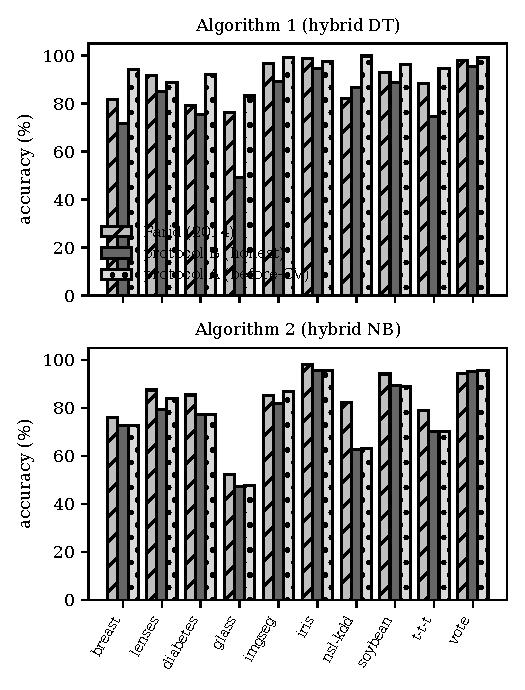
\includegraphics[width=3.4in]{figures/fig1_r1_protocols.pdf}
\caption{Accuracy of Algorithm~1 (top) and Algorithm~2 (bottom) per
dataset: Farid et al.'s reported number, protocol B (refit-per-fold,
honest), and protocol A (fit-before-CV). Algorithm~1's protocol-A bars are
inflated on almost every dataset; Algorithm~2's three series stay close
together.}
\label{fig:r1_protocols}
\end{figure}

\subsection{The filter hurts a downstream tree, and order barely matters}

Table~\ref{tab:e9} reports E9's protocol-B pipeline results. Chaining
Algorithm~1 into a final tree costs accuracy relative to the no-cleaning
baseline (80.58\% vs.\ 85.16\% mean, both final DT), and the cost is not
uniform across datasets: Fig.~\ref{fig:removal} plots, per dataset, the
percentage of training rows Algorithm~1 removes against the resulting
change in the tree's accuracy relative to the baseline tree. The largest
drop is on tic-tac-toe ($-18.18$ points), and the only clear gain is on
breast-cancer ($+5.45$ points), consistent with a filter that helps only
where the NB judge is a better error detector than the tree already is on
its own, and otherwise discards rows the tree needed. Algorithm~2's effect
on the tree is close to neutral (85.01\% vs.\ 85.16\%), consistent with a
tree re-deriving similar splits from whichever 69.97\% of attributes
survive selection on average. Swapping the order of the two algorithms
changes accuracy by less than one point on both final classifiers: Path~2
minus Path~1 has a median difference of $-0.09$ points for a final tree
($p=0.846$) and $+0.97$ points for a final NB ($p=0.322$), neither
significant even before correction. Order is not the lever that recovers
the paper's reported gains.

% E9: refit-per-fold, 10-fold CV x 5 seeds, alpha=0, mixed NB, weights on.
\begin{table}[t]
\caption{E9 pipeline, mean accuracy over 10 datasets ($\pm$ across-dataset SD), 10-fold CV $\times$ 5 seeds.}
\label{tab:e9}
\centering\small
\begin{tabular}{lrr}
\toprule
Arm & final DT & final NB \\
\midrule
baseline (no cleaning) & 85.16 $\pm$ 13.42 & 77.82 $\pm$ 14.13 \\
Algorithm 1 alone & 80.58 $\pm$ 13.41 & 76.58 $\pm$ 16.38 \\
Algorithm 2 alone & 85.01 $\pm$ 13.38 & 76.45 $\pm$ 14.33 \\
Path 1 (Alg1 $\to$ Alg2) & 80.52 $\pm$ 13.49 & 76.15 $\pm$ 16.70 \\
Path 2 (Alg2 $\to$ Alg1) & 79.54 $\pm$ 14.09 & 75.89 $\pm$ 14.77 \\
\bottomrule
\end{tabular}
\end{table}


\begin{figure}[t]
\centering
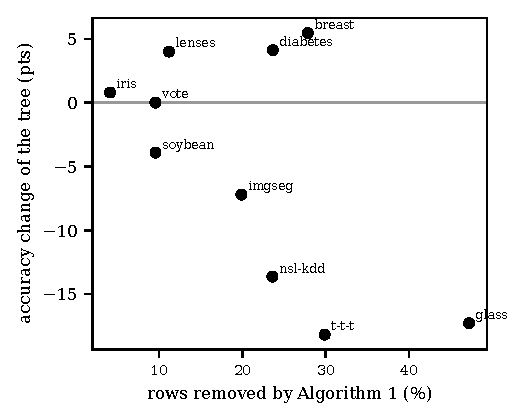
\includegraphics[width=3.4in]{figures/fig2_alg1_removal_vs_tree.pdf}
\caption{Rows Algorithm~1 removes (mean over folds and seeds, x-axis)
against the change in the downstream tree's accuracy relative to the
no-cleaning baseline (y-axis), one point per dataset. Datasets where the
filter removes a large share of rows tend to see the tree's accuracy fall.}
\label{fig:removal}
\end{figure}

% Wilcoxon signed-rank tests over the 10 datasets, Holm-adjusted within this family of 8 (n=10, low power; Demsar 2006).
\begin{table}[t]
\caption{Wilcoxon signed-rank tests over the 10 datasets (n=10 pairs unless noted; two-sided; Holm-adjusted p within this table).}
\label{tab:tests}
\centering
\small
\setlength{\tabcolsep}{3pt}
\begin{tabular}{lrrrr}
\toprule
Comparison & $W$ & $p$ & med.\ diff.\ & Holm $p$ \\
\midrule
R1 protocol A vs B, Alg1 & 0.0 & 0.002 & +11.58 & 0.016 \\
R1 protocol A vs B, Alg2 & 10.0 & 0.164 & +0.14 & 0.656 \\
E3a protocol A vs B, Alg1 & 0.0 & 0.002 & +15.52 & 0.016 \\
E3a protocol A vs B, Alg2 & 9.0 & 0.129 & +0.29 & 0.645 \\
R1 honest Alg1 vs C4.5 & 6.0 & 0.055 & -3.71 & 0.328 \\
R1 honest Alg2 vs NB & 10.0 & 0.164 & +0.65 & 0.656 \\
E9 Path 2 vs Path 1, final DT & 25.0 & 0.846 & -0.09 & 0.846 \\
E9 Path 2 vs Path 1, final NB & 17.0 & 0.322 & +0.97 & 0.656 \\
\bottomrule
\end{tabular}
\end{table}

